\label{clustering}
One of the goals of this thesis was to visualize the structure of the scraped portion of the dark web. We chose to render the data as a web graph which is further outlined in Section~\ref{webGraph}. As was described in Chapter~\ref{datasetAnalysis}, the data set to be displayed was rather sizable. The problem with the visualization of such an amount of data is readability. All pages of such a data set cannot be displayed at the same time if additional information, such as the category with the url address of the page, need to be provided to the user. Such rendering would be cluttered and readability would be affected negatively. It was therefore necessary to find a proper way to divide the graph into several subgraphs. We decided to adopt community structure introduced in Section~\ref{communityStructure}. For community detection we leveraged two algorithms for comparison purposes. One of them is the well known Louvain algorithm (LA). LA is outlined in more detail in Section~\ref{louvainAlgorithm}. The other one is the Leiden algorithm (LeA), an improved version of LA. LeA is described in Section~\ref{leidenAlgorithm}.

In this chapter we characterize web graphs and their challenges. Next we talk about community structure and LA, the algorithm for dividing a graph into communities. 
 
\section{Web graph} \label{webGraph}
The data are displayed as a web graph~\cite{the_web_graph_overview}. A web graph is a graph representation of the web. Nodes are portrayals of the pages and edges depict links between the pages. Web graphs tend to be built from an enormous amount of data. As such, they can be advertised in various ways. One of the visualizations is shown in Figure~\ref{hugeWebGraphFireworks}. 
\begin{figure}[ht!]
  \centering
  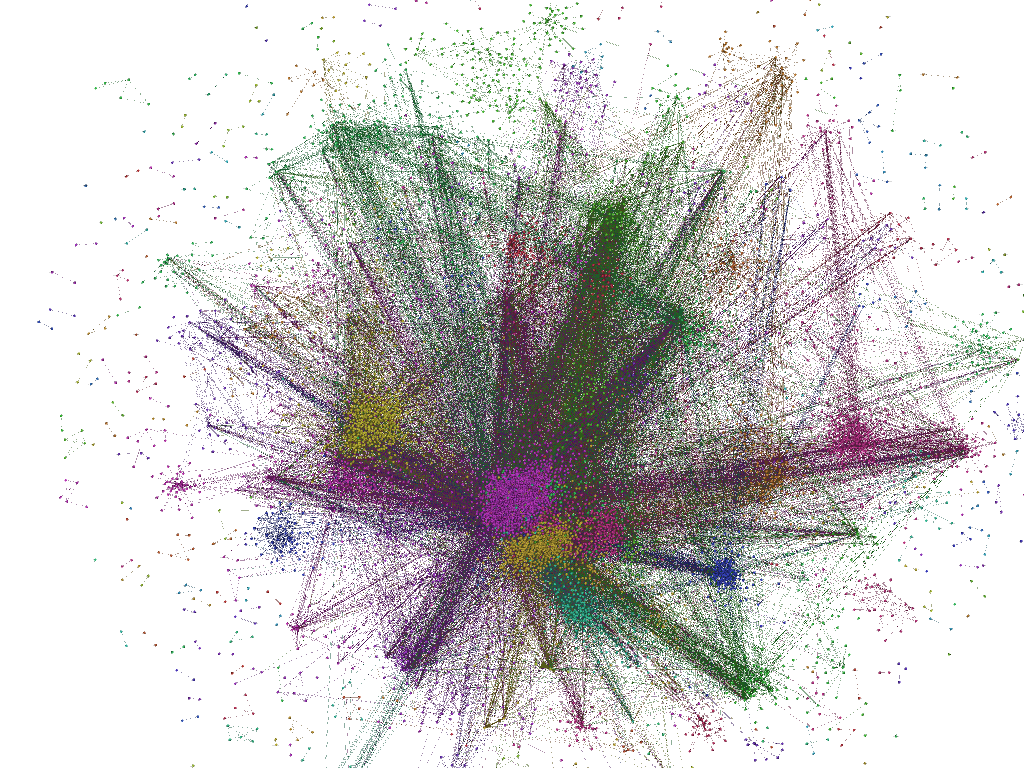
\includegraphics[width=\textwidth]{Images/hugeWebGraphFireworks.png}
  \caption{Web graph made by Citeo consisting of circa 600 000 domains and 16 billion links.~\cite{hugeWebGraphFireworks}.}
  \label{hugeWebGraphFireworks}
\end{figure} 
The depicted web graph displays all its data at once without any labels or details. The result may be useful for viewing the internet as a whole. However, for our purposes this view was not sufficient. One of the goals of this thesis was the possibility of the inspection of the relationships between nodes in more detail. The big amount of data described in Subsection~\ref{dataSet} prevented the displaying of all pages at once. The information the user would read from such a graph would be either incompatible with the requirements or incomprehensible as too much visual data worsens the quality of the user's information processing~\cite{informationCluttering}. Therefore the requirement arose for the graph to be composed of a significantly smaller amount of nodes. As a result the user would be able to obtain the sought knowledge without hindrance. A considerable amount\footnote{Out of 210,191 node 90,275 were connected and 119,916 were isolated.} of nodes in our graph were not isolated\footnote{An isolated node is a node with zero incoming and outgoing edges.}. Those nodes were in fact part of a single connected component. It was therefore possible to partition the graph based on the density of its nodes into communities. Communities are characterized in detail in the next Subsection~\ref{communityStructure}.

\subsection{Community structure} \label{communityStructure}
If a graph can be partitioned into several subgraphs so that nodes from one subgraph are internally connected densely and are connected scarcely to nodes from other subgraphs, we can claim it has a community structure. Each subgraph of such a graph is a community~\cite{communitiesOverview}. Each community can be portrayed as a meta node of the graph. This way the number of nodes in the graph is reduced. The quality of such a partition is measured using modularity. L. Wenye and D. Schuurmans describe modularity in their work~\cite{modularityOverview} with the following words: \begin{quotation}  For a candidate partition of the vertices into clusters, the modularity is defined to be the portion of the edge connections within the same cluster minus the expected portion if the connections were distributed randomly~\cite{modularityDefinition}. \end{quotation} Modularity is represented by a number between -1 and 1. If the value is positive the connections between nodes of the same cluster are more densely connected than the randomly distributed connections between the same nodes.

\section{Louvain algorithm} \label{louvainAlgorithm}
A widely used algorithm for finding communities in graphs is the LA~\cite{louvainAlgorithm}. It is a greedy algorithm which maximizes modularity locally. In this algorithm, modularity is an indicator of the density of connections between nodes belonging into the same communities as opposed to links between communities. The modularity calculation is also taking into account whether the graph is weighted\footnote{A graph in which the links have weights assigned to them.} or not.

Next we detail the principle of the algorithm. We example each step on node $N_{A}$ belonging to a portion of an example graph illustrated in Figure \ref{exampleGraphLouvain}.
\begin{figure}[ht!]
  \centering
  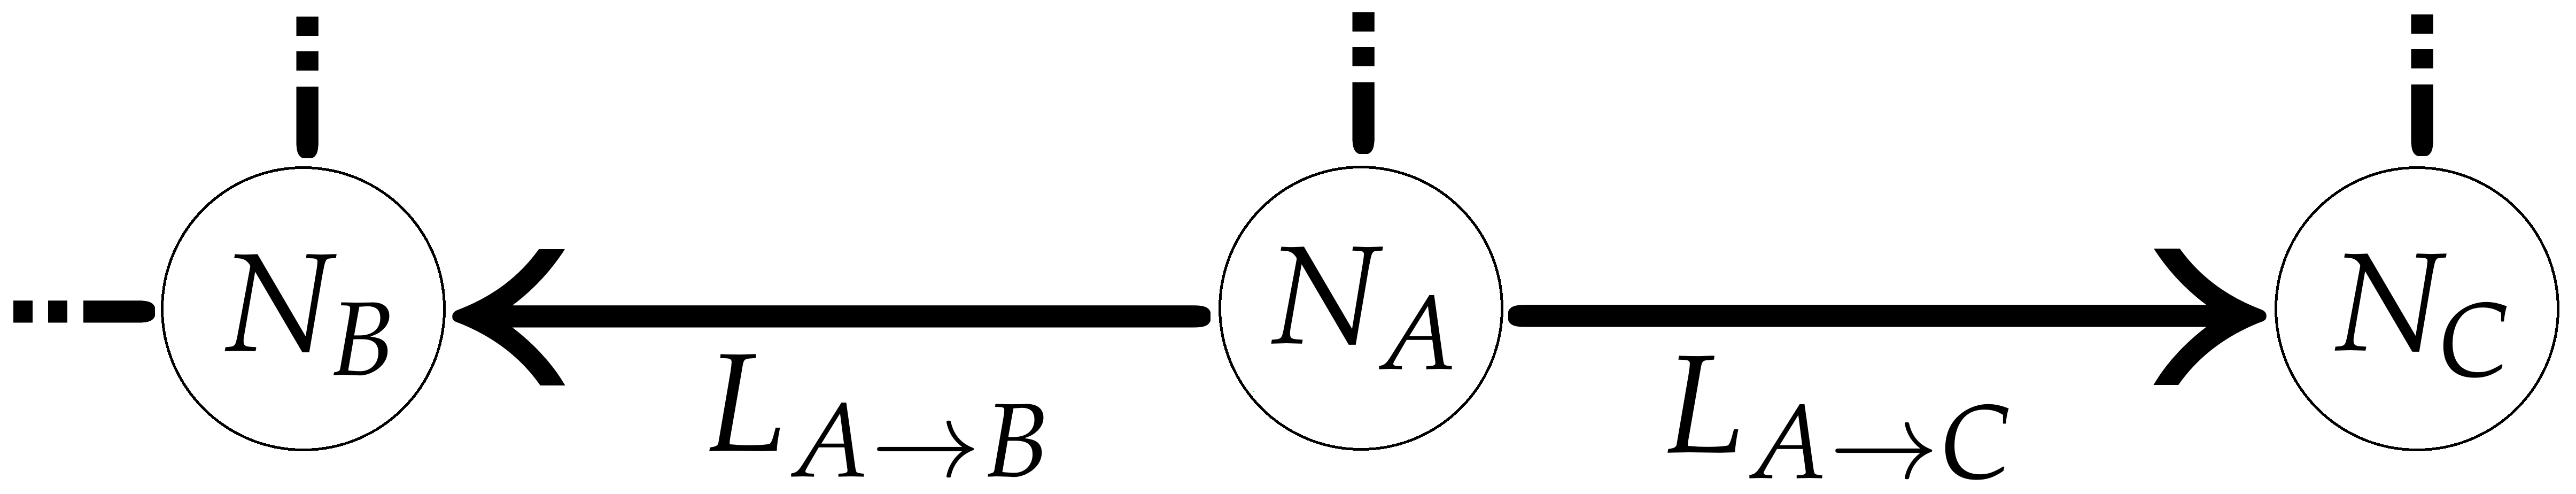
\includegraphics[width=\textwidth]{Images/graphForCommunity.png}
  \caption{The visible portion of the exampled graph depicts nodes $N_{A}$, $N_{B}$, and  node $N_{C}$. There are links  $L_{A\rightarrow B}$ and  $L_{A\rightarrow C}$  between nodes  $N_{A}$ and  $N_{B}$, and  $N_{A}$ and  $N_{C}$ respectively. Other links are displayed partially and are connecting the nodes to the rest of the graph.}
  \label{exampleGraphLouvain}
\end{figure} 

\begin{enumerate} [label=\alph*)]
  \label{louvainAlgorithmPrinciple}
  \item  Each node is assigned a community. Current modularity for each node is calculated. 
  \label{LA1}
  \begin{itemize}
    \item Node $N_{A}$ is assigned to community $C_{A}$. Let us assume modularity $M_{A\rightarrow cA}$ for $N_{A}$ is \textit{0.2}.
  \end{itemize} 
  \item Each node is disassociated from its community and randomly appointed to a community of one of its neighbours. This is repeated for each neighbour of the node. Modularity for each node after each such a transition is calculated.
  \label{LA2}
  \begin{itemize}
    \item Node $N_{A}$ has two neighbouring nodes, node $N_{B}$ in community $C_{B}$ and node $N_{C}$ in community $C_{C}$. Node $N_{A}$ is removed from $C_{A}$ and appointed to $C_{B}$. Let us say modularity $M_{A\rightarrow cB}$ is \textit{-0.1}. Afterwards, $N_{A}$ is removed from $C_{B}$ and assigned to $C_{C}$. Let us suppose modularity $M_{A\rightarrow cC}$ is \textit{0.5}. 
  \end{itemize} 
  \item Each node is now appointed to the community in which the maximum modularity was achieved. This can also result in the node remaining in its original community.
  \label{LA3}
  \begin{itemize}
    \item The maximum modularity of $N_{A}$ achieved in the previous step is $M_{A\rightarrow cC}$. $N_{A}$ is therefore removed from $C_{A}$ and appointed to $C_{C}$.
  \end{itemize} 
  \item Discard the empty communities. 
  \label{LA4}
  \begin{itemize}
    \item Community $C_{A}$ is now empty and is therefore discarded.
  \end{itemize} 
  \item Each community is now considered a node (community-node). Links between community-nodes are constructed from links of nodes of the same community-node (old-links). This is done by grouping together old-links which target nodes assigned to the same target community-node. These grouped links now represent weighted edges between community-nodes. Old-links between nodes of the same community-node are represented  by a self-loop on the community-node.
  \label{LA5}
  \begin{itemize}
    \item Community $C_{C}$ is now considered a node $N_{cC}$ and $C_{B}$ is considered a node $N_{cB}$. Link $L_{cC\rightarrow cB}$ from $N_{cC}$ to $N_{cB}$ with a weight of 1 is created because  of link $L_{A\rightarrow B}$. Also, a loop $L_{cC\rightarrow cC}$ is created on $N_{cC}$ because of the link $L_{A\rightarrow C}$. The result of this step can be observed in Figure \ref{exampleGraphLouvainEnde}.
  \end{itemize}  
  \begin{figure}[ht!]
    \centering
    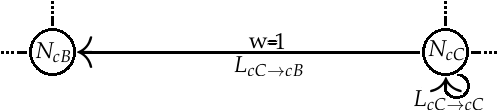
\includegraphics[width=\textwidth]{Images/graphForCommunityEnde.png}
    \caption{This graph is the result of applying the above listed steps to the previously shown portion of the example graph from Figure \ref{exampleGraphLouvain}. The visible portion of the graph contains nodes $N_{cB}$ and $N_{cC}$, and a link $L_{cC\rightarrow cB}$ with a weight of 1 between them. A self-loop $L_{cC\rightarrow cC}$ on $N_{cC}$ is present.}
    \label{exampleGraphLouvainEnde}
\end{figure}     
\end{enumerate}
The above detailed steps are repeated until modularity is not improved any more.

The LA is favoured for its simplicity, speed and accuracy. Since its introduction, in 2008, it was possible to detect communities in graphs with billions of nodes in a relatively timely manner. 

The LA was compared to other algorithms for community detection \cite{louvainAlgorithm}.  Namely the algorithm of Wakita and Tsurumi \cite{wakitaAndToshiyuki}, the algorithm of Pons and Latapy \cite{ponsAndLatapy}, and the algorithm of Clauset, Newman and Moore \cite{CNM}. The used graphs were of sizes varying between 34 nodes and 77 edges to as much as 118 million nodes and 1 billion edges. The difference between the computing times of the previously stated algorithms grew with the size of the graphs and favours LA. In fact, it took 152 minutes for the LA to detect the communities of the greatest graph whereas the computation time of the other algorithms was more than 24 hours. In terms of precision, LA was also the most precise one with slightly better modularities.


\section{Leiden algorithm} \label{leidenAlgorithm}
The LeA is another algorithm for community detection on large graphs. The authors of the LeA claim the LA to have a major flaw \cite{leidenAlgorithm}. The LA may detect badly connected, or internally disconnected communities\footnote{It is not possible to form a connected component from nodes of an internally disconnected community.}. The latter phenomenon occurs when a bridge-node\footnote{A node connecting two or more connected components otherwise not connected between each other.} of one community is assigned to another community and the remaining nodes are not. The LeA is based on the LA and eliminates the before mentioned problems. 

Next we outline the principle of the LeA. The detailed steps are portrayed in Figure \ref{leidenVisualization} \cite{leidenVisualization}. The steps are compared to the steps depicted in the characterization of the LA in Section \ref{louvainAlgorithm} and described using the visualization.
\begin{figure}[ht!]
  \centering
  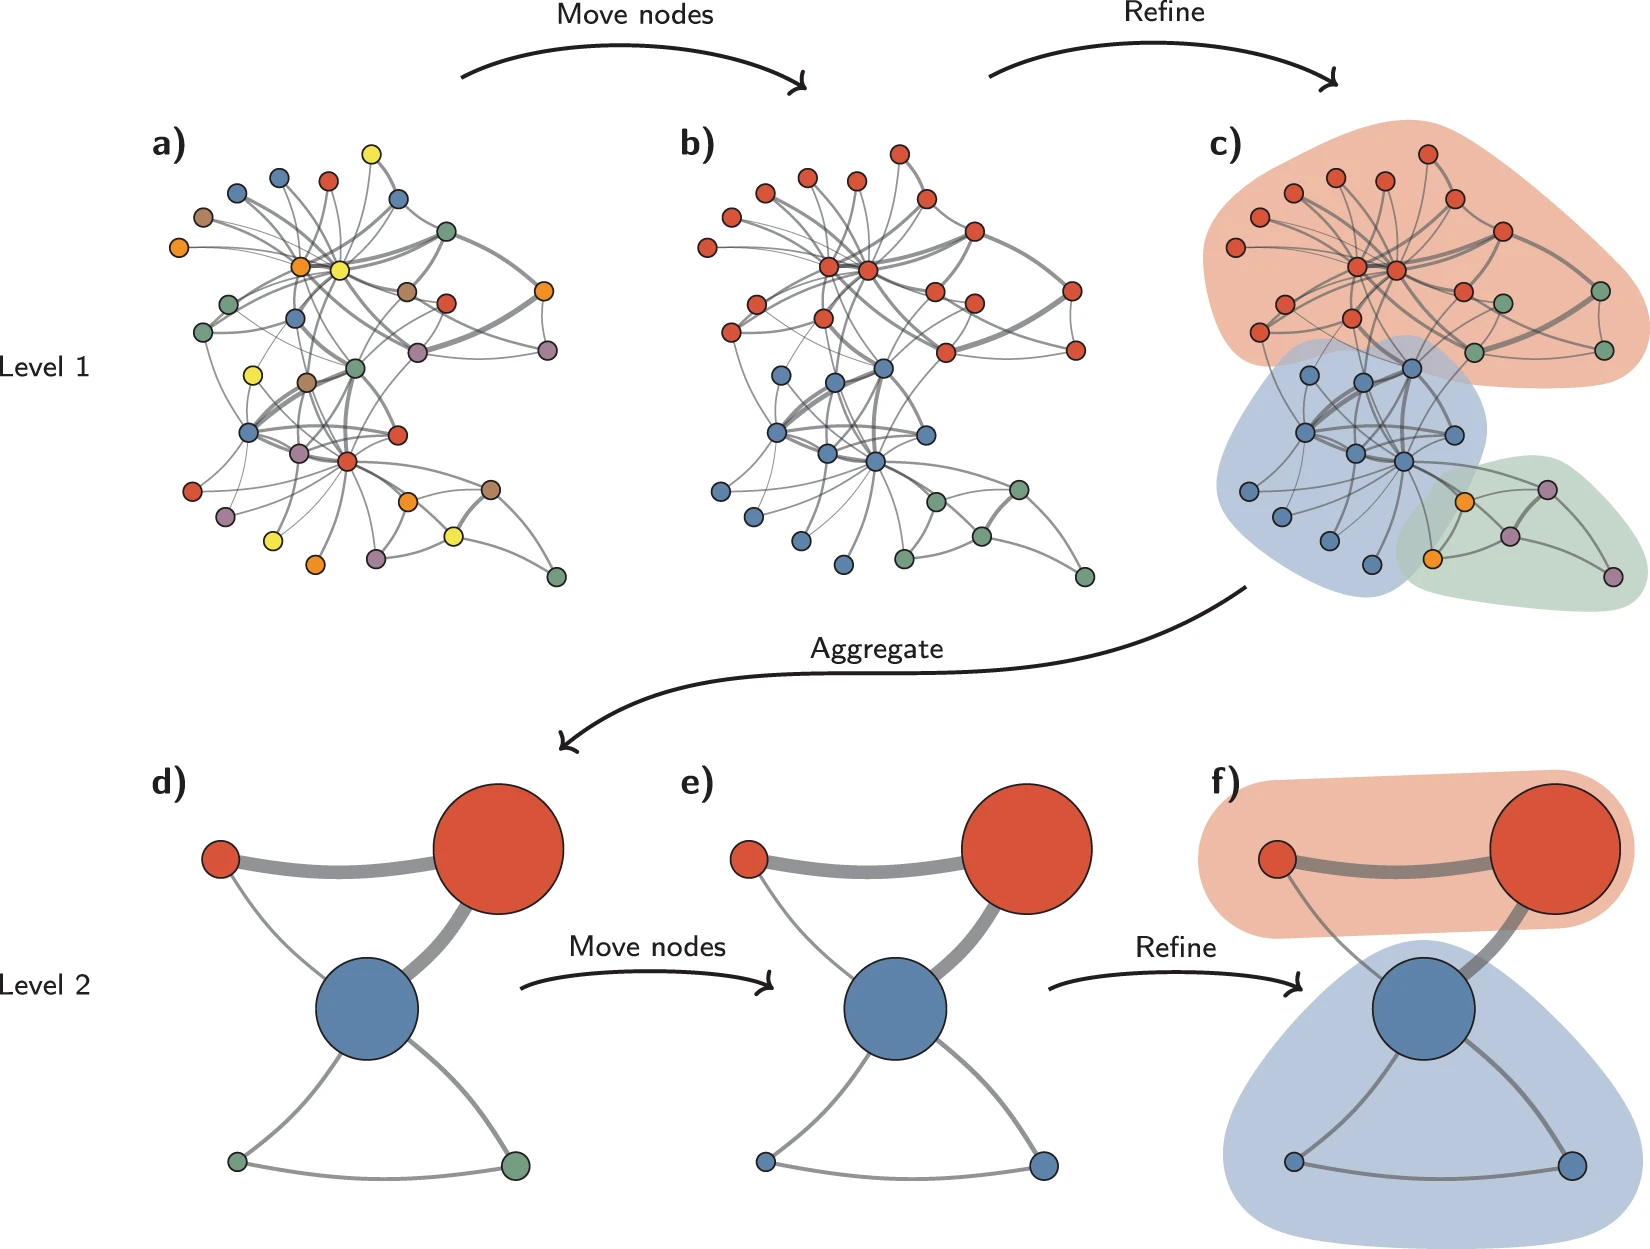
\includegraphics[width=\textwidth]{Images/leidenVisualization.png}
  \caption{The visualization of the principle of the LeA \cite{leidenVisualization} by the authors of \textit{From Louvain to Leiden: guaranteeing well-connected communities} \cite{leidenAlgorithm}. Steps \textit{a)} to \textit{d)} are described in the above included characterization. Steps \textit{e)} and \textit{f)} show a part of a second iteration of the algorithm. The algorithm ended in step \textit{f)} because no further improvement was achieved by \textbf{refining} the communities.}
  \label{leidenVisualization}
\end{figure}    
 
\begin{enumerate}[label=\alph*)]
  \item This phase corresponds to step LA~\ref{LA1}. 
  \begin{itemize}
    \item \textit{(Figure \ref{leidenVisualization}) a)}. Each node is assigned a community. This is portrayed by the nodes being of different colours. \label{leidenAlgorithmPrincipleA}
  \end{itemize} 
    \label{LeAa}
  \item This phase is called \textbf{move nodes} and corresponds to steps \textit{LA~\ref{LA2}}, \textit{LA~\ref{LA3}}, and \textit{LA~\ref{LA4}}. 
  \begin{itemize}
    \item \textit{(Figure \ref{leidenVisualization}) b)}. The nodes are divided into three communities represented by the colours of the nodes - a red, a blue and a green one. \label{leidenAlgorithmPrincipleB}
  \end{itemize} 
    \label{LeAb}
  \item This phase is called \textbf{refine}. Steps \textit{LA~\ref{LA1}} and \textit{LA~\ref{LA2}} are applied to nodes within communities. This results into the further partitioning of communities into sub-communities.
  \begin{itemize}
    \item \textit{(Figure \ref{leidenVisualization}) c)}. The communities are refined within communities. The red community was refined into two sub-communities - a red-red one and a red-green one. The blue community was not refined further. The green was refined into a green-orange one and a green-purple one. 
  \end{itemize} 
    \label{LeAc}
  \item This phase is called \textbf{aggregation} and corresponds to step \textit{LA~\ref{LA5}}  but sub-communities are treated as communities. Nodes created from sub-communities within one community are considered to belong to the same community. This consideration is taken into account in further iterations. Otherwise, these nodes are regarded as individual nodes. This practice prevents bridge-nodes to be appointed to a different community and so disconnect the former community.
  \begin{itemize}
    \item \textit{(Figure \ref{leidenVisualization}) d)}. The sub-communities are considered nodes now. However, sub-communities from the same community are still considered to belong together. Therefore the colours of the nodes corresponds to the colours of the communities from the previous step. 
  \end{itemize} 
    \label{LeAd}
\end{enumerate}
These steps are repeated until no further improvement in modularity can be achieved. 

Step \ref{LeAd} is in further iterations significant.  It is impossible to re-assign a bridge-node to a different community with the LeA. But this may happen using the LA. Now we demonstrate why on Figure~\ref{leidenVisualization}~\textit{f)}. 

A bridge node in the blue community connecting the two smaller nodes is depicted. Let us call this bridge-node \textit{B}. With the LeA, all blue nodes are still considered to be of the same community. Therefore they cannot be shifted into any neighbouring communities. 

Let us now assume we ran another iteration of the LA over the graph in Figure~\ref{leidenVisualization}~ \textit{f)}. The blue nodes are not considered belonging to the same community anymore. The nodes are viewed as unrelated neighbouring nodes. There is therefore a possibility for node \textit{B} to be assigned to the red community if higher modularity is achieved. This would leave the two smaller blue nodes disconnected. 

In this thesis implementations of both, the LA and the LeA, were used.